% 02.06.2016 12:00 CET last changed by a.holzinger
% General Template for LNCS and LNAI contributions based on llncs, adapted by ah
% Many thanks to the TRS team
% In case of using eps compile via 1) TeXify and then proceed with 2) dvi2pdf
%
\documentclass{llncs}
\usepackage{float}

\usepackage[dvips]{graphicx}
\usepackage[ruled,vlined]{algorithm2e}
\usepackage{amsfonts}
\usepackage{amssymb}
\usepackage{amsmath}
\usepackage{mathtools}

\providecommand{\abs}[1]{\lvert#1\rvert}
\providecommand{\norm}[1]{\lVert#1\rVert}

\usepackage{calc}
\usepackage{subfigure}

\usepackage{color}
\usepackage{soul}
\usepackage{comment}

\newtheorem{prop}{Property}

\newenvironment{Bitemize}{\renewcommand\labelitemi{\textbullet}\begin{itemize}}{\end{itemize}}

\begin{document}

\title{Interactive Anonymization\\
for Privacy aware Machine Learning}

\author{Bernd Malle\inst{1}\inst{2}, Peter Kieseberg\inst{1}\inst{2}, Andreas Holzinger\inst{1}}

\institute{Holzinger Group HCI-KDD \\
Institute for Medical Informatics, Statistics \& Documentation\\
            Medical University Graz, Austria\\
            \texttt{b.malle@hci-kdd.org}
\and
SBA Research gGmbH, Favoritenstraße 16, 1040 Wien \\
			\texttt{PKieseberg@sba-research.org}
}
	
\maketitle

% ==================================
%				ABSTRACT
% ==================================
\begin{abstract}




\medskip

\textbf{Keywords}: Machine Learning, Privacy aware ML, interactive ML, Knowledge Bases, Anonymization, k-Anonymity, SaNGreeA, Information Loss, Weight Vectors


\end{abstract}

\renewcommand{\thesubfigure}{\thefigure.\arabic{subfigure}}
\makeatletter
\renewcommand{\p@subfigure}{}
\renewcommand{\@thesubfigure}{\thesubfigure:\hskip\subfiglabelskip}
\makeatother


% ==================================
%			INTRODCUTION
% ==================================
\section{Introduction and Motivation}
\label{sect:intro_moti}


% ==================================
%			    PAML
% ==================================
\section{Privacy aware Machine Learning}
\label{sect:paml}


% ==================================
%			  PRIVACY
% ==================================
\section{Methods of providing privacy}
\label{sect:methods_privacy}

\subsection{Perturbation}
\label{ssect:perturbation}

\subsection{$\epsilon$  differential privacy}
\label{ssect:eps_priv}

Introduce randomness into the data.. can never be sure if specific answer is correct, nevertheless a certain fraction of ansers will statistically be correct.

Laplace (double exponential) distribution.. close to 0 - large perturbation - further out smaller ...

\subsection{k-anonymity (and beyond)}
\label{ssect:k_anon}

Figure~\ref{fig:anon_categories} illustrates the original tabular concept of anonymization: Given an input table with several columns, we will in all probability encounter three different categories of data:


\begin{figure}[!t]
	\begin{center}
		%		\includegraphics[width=\textwidth]{figures/anonym/gen_hierarchy}
		\caption{Example of a typical generalization hierarchy}
		\label{fig:gen_hierarchy}
		\small
		taken from \cite{aggarwal2005approximation}
	\end{center}
\end{figure}


\begin{itemize}
	\item \textbf{Personal identifiers} are data items which directly identify a person without having to cross-reference or further analyze them. Examples are email address or social security number (SSN). As personal identifiers are immediately dangerous, this category of data is usually removed.
	\item \textbf{Sensitive data,} also called 'payload', represents information that is crucial for further data mining or research purposes. Examples for this category would be disease classification, drug intake or personal income. This data shall be preserved in the anonymized dataset and can therefore not be deleted or generalized.
	\item \textbf{Quasi identifiers (QI's)}, are data which in themselves do not directly reveal the identity of a person, but might be used in aggregate to reconstruct it. For instance, \cite{sweeney2002k} reported in 2002 that the identity of 87\% of U.S. citizens could be uncovered via just the 3 attributes \textit{zip code}, \textit{gender} and \textit{date of birth}. Despite this danger, QI's may contain vital information to research applications (like ZIP code in a disease spread study); they are therefore generalized to an acceptable compromise between privacy (data loss) and information content (data utility).
\end{itemize}



% ==================================
%				iML
% ==================================
\section{interactive Machine Learning}
\label{sect:iML}

Interactive ML algorithms adjust their inner workings by continuously interacting with an outside \textit{oracle}, drawing positive / negative reinforcement from this interaction \cite{2016HolzingeriML}. Such systems are especially useful for highly-personalized predictions or decision support \cite{2016KiesebergDITL}; moreover many real-world problems exhibit (super)exponential algorithmic runtime; in such cases human brains dwarf machines at approximating solutions and learning from very small samples, thus enabling us to 'intuit' solutions efficiently \cite{2016iMLExperiment}.

By incorporating humans as oracles into this process, we can elicit background knowledge regarding specific use cases unknown to automatic algorithms \cite{WARE2001}. This however is highly dependent on the users' experience in a certain field as well as data / classification complexity; domain experts can of course be expected to contribute more valuable decision points than laymen; likewise, a low-dimensional dataset and simple classification tasks will result in higher quality human responses than convoluted problem sets.

While the authors of \cite{Moque2012} propose a system that interacts with a user in order to set a certain k-factor and subsequently provides a report on information loss and Kurtosis of QI distributions, the algorithm is not \textit{interactive} by our definition in that it does not influence the inner workings of the algorithm during the learning phase. This is also true in case of the Cornell Anonymization Toolkit (Cat) \cite{Xiao2009}, which conducts a complete anonymization run and only then lets the user decide if they are content with the results. In contrast, our approach alters algorithmic parameters upon every (batch of) human decisions, letting the algorithm adapt in real-time.

\cite{Loh2010} describe an approach incorporating humans into the anonymization process by allowing them to set constraints on attribute generalization; moreover they construct generalization hierarchies involving domain-specific ontologies. Although this technique marks a departure from wholesale automatic anonymization, it still lacks the dynamic human-computer interaction of our approach.

Apart from the field of privacy, interactive ML is today present in a wide spectrum of applications, from bordering medical fields like protein interactions / clusterings \cite{Amershi2014} via on-demand group-creation in social networks \cite{Amershi2012} to even teaching algorithms suitable mappings from gestures to music-generating parameters \cite{Fiebrink2009}.


% ==================================
%			EXPERIMENTS
% ==================================
\section{Experiments}
\label{sect:experiments}

The following sections will describe our experiment in detail, encompassing the data source selected, the algorithm used as well as a description of the overall process employed to obtain our results.


\subsection{Data} 
\label{ssect:data}

We chose the adults dataset from the UCI Machine Learning repository which was generated from US census data of 1994 and contains approximately 50k entries; of those 30,162 were selected after preprocessing. Of the attributes (data columns) provided only one was deleted because it was also represented by a column containing its numerical mapping (education $=>$ education\_num). Figure~\ref{fig:adult_original_distribution} shows the attribute value distribution of the original input dataset with the exception of the sample weights.



\subsection{Algorithm}
\label{ssect:algorithm}

SaNGreeA stands for \textit{Social network greedy clustering} and was introduced by \cite{campan2009data}. In addition to 'clustering' nodes of a graph according to the minimum general information loss (GIL) incurred as described in Section~\ref{ssect:tab_anonym}, this algorithm also considers the structural information loss (SIL) incurred in assigning a node to a certain cluster. The SIL quantifies the probability of error when trying to reconstruct the structure of the initial graph from its anonymized version.

\begin{equation*}
\begin{split}
\text{GIL}(cl) = \abs{cl} \cdot (\sum_{j=1}^{s} \frac{size(gen(cl)[N_j])}{size(min_{x \epsilon N} (X[N_j]), max_{x \epsilon N} (X[N_j]))} \\
+ \sum_{j=1}^{t} \frac{height(\Lambda(gen(cl)[C_j]))}{height(H_{C_j})})
\end{split}
\end{equation*}


where:\\
- $\abs{cl}$ denotes the cluster cl's cardinality; \\
- $size([i1,i2])$ is the size of the interval $[i1,i2]$, i.e., $(i2-i1)$; \\
- $\Lambda(w), w \epsilon H_{C_j}$ is the sub-hierarchy of $H_{C_j}$ rooted in $w$; \\
- $height(H_{C_j})$ denotes the height of the tree hierarchy $H_{C_j}$; \\


The total generalization information loss is then given by:
\begin{equation*}
\text{GIL}(G,S) = \sum_{j=1}^{v} \text{GIL}(cl_j)
\end{equation*}
And the normalized generalization information loss by:
\begin{equation*}
\text{NGIL}(G,S) = \frac{\text{GIL}(G,S)}{n \cdot (s+t)}
\end{equation*}

The main process...


\subsection{Process}
\label{ssect:process}

To examine the impact of perturbation and anonymization of datasets on the quality of a classification result, we designed the following processing pipeline:


\begin{enumerate}
	\item Taking the original (preprocessed) dataset as input, we transformed its attributes to boolean values, so instead of \textit{native-country $->$ United-States} we considered \textit{United-States $->$ yes / no}.
	% \item A correlation matrix of the resulting binary feature set was computed to get a better feeling for the data (see Figure~\ref{fig:adult_correlation_big}).
	\item We then ran 4 different classifiers on it and computed precision, recall as well as F1 score. The four classifiers used were \textit{gradient boosting}, \textit{random forest}, \textit{logistic regression} and \textit{linear SVC}.
	\item From the obtained results we extracted the 3 attribute values most contributing to a "positive" ($>$50k) result as well as the top 3 attribute values indicating a "negative" ($<=$50k) prediction as depicted in Figure~\ref{fig:adult_important_columns}
	\item For each of these 6 attribute values, we subsequently deleted a specific percentage of data rows containing that value from the original dataset, resulting in 30 reduced datasets. The 5 percentages used were $0.2$, $0.4$, $0.6$, $0.8$ as well as $1.0$.
	\item To each of those datasets we re-applied the four chosen classifiers successively and recorded the respective impact on the quality of the classification result. The results can be seen in Figure~\ref{fig:adult_results_perturbation_top} and Figure~\ref{fig:adult_results_perturbation_bottom}.
	\item In order to measure the effects of k-anonymization on classifier performance, we used the SaNGreeA's GIL component described in the following section to generate datasets with a k-factor of $k=3$, $k=7$, $k=11$, $k=15$ as well as $k=19$. Furthermore, we used each of these settings with 3 different weight vectors: 1) equal weights for all attributes, 2) age information preferred ($\omega(age)=0.88$, $\omega(other\_attributes)=0.01$) and 3) race information preferred ($\omega(race)=0.88$, $\omega(other\_attributes)=0.01$). We then re-executed all classifiers on the resulting 15 datasets and recorded the respective results, which can be seen in Figure~\ref{fig:adult_results_anonymization}.
\end{enumerate}


\begin{figure}[!t]
	\begin{center}
		\vspace{-1.0cm}
    	\hspace*{-0.8cm}
		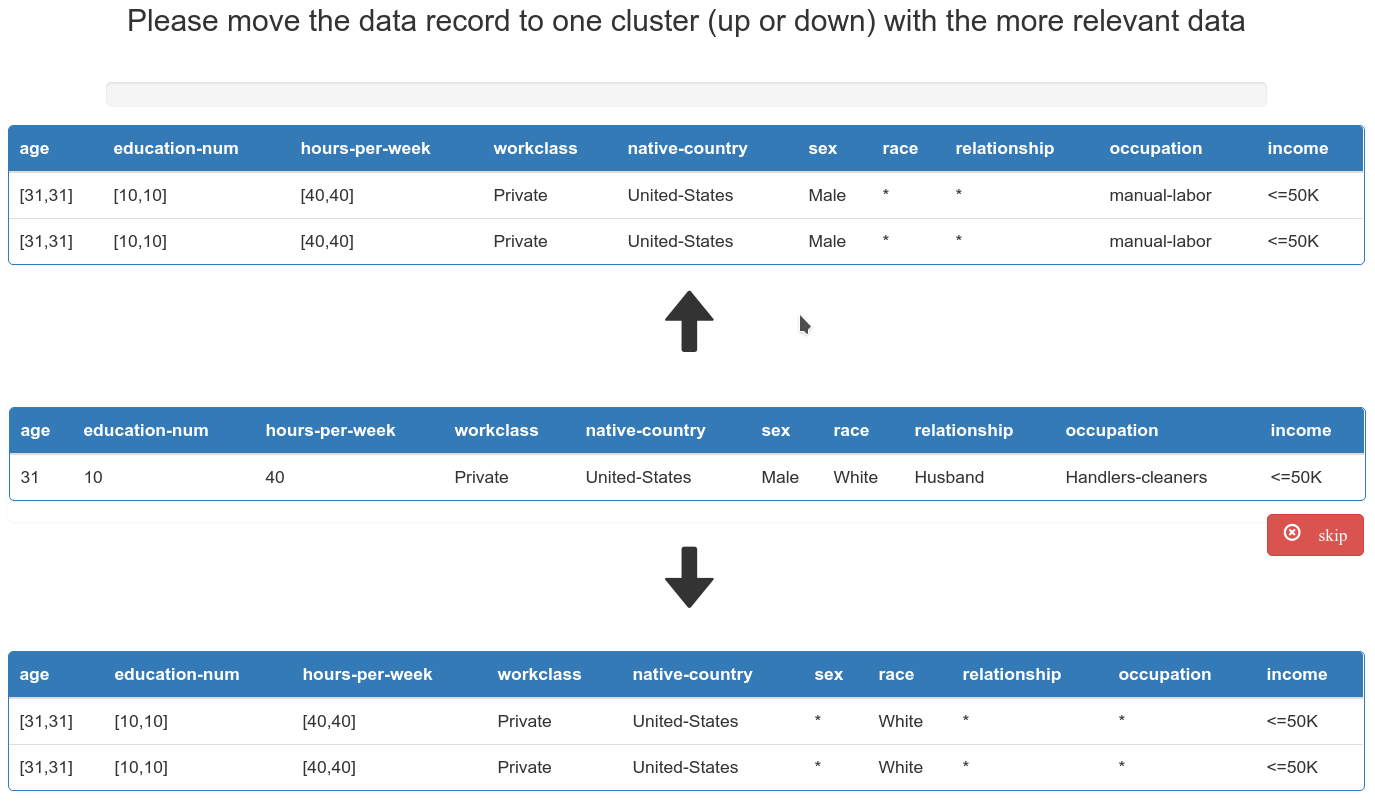
\includegraphics[width=1.0\textwidth]{figures/iml_anon_screen1}
		
		\vspace{1.0cm}
		\hspace*{-0.8cm}
		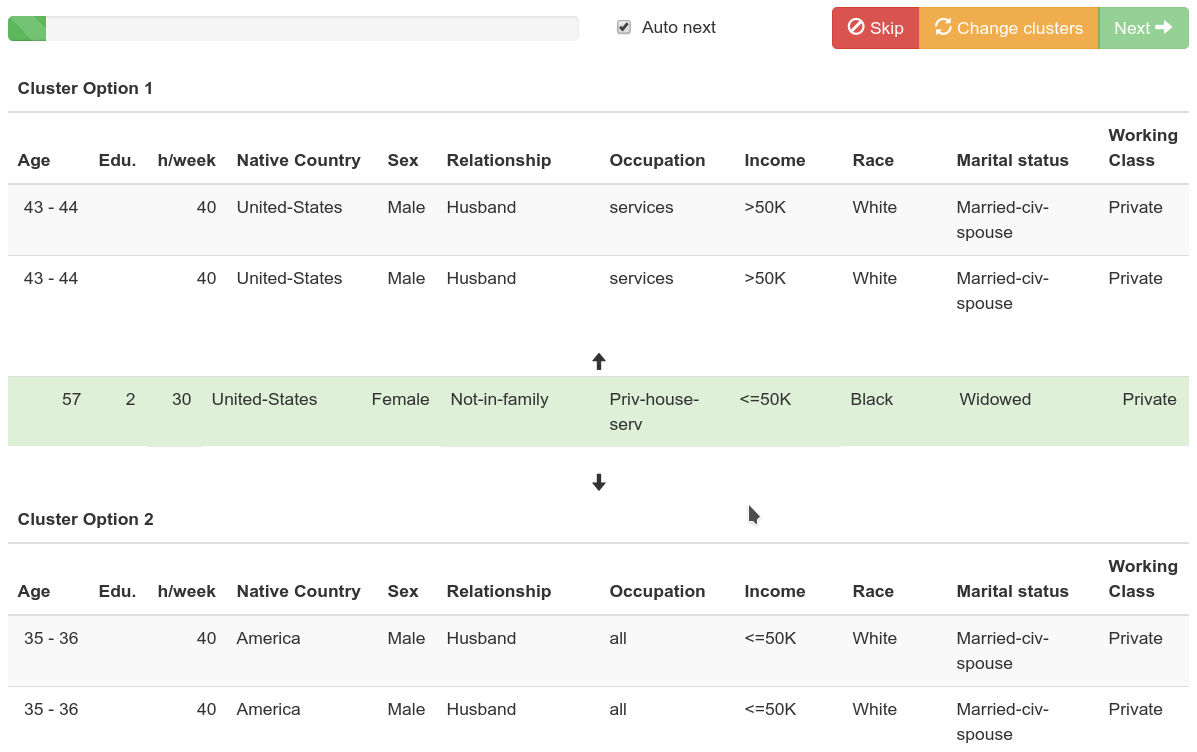
\includegraphics[width=1.0\textwidth]{figures/iml_anon_screen2}
		\caption{Two implementations of the iML interface design...}
		\label{fig:adult_important_columns}
	\end{center}
\end{figure}


% ==================================
%		RESULTS & DISCUSSION
% ==================================
\section{Results \& Discussion}
\label{sect:results}

\begin{figure}[!h]
	\begin{center}
		\vspace{-1.0cm}
		\hspace*{-0.8cm}
		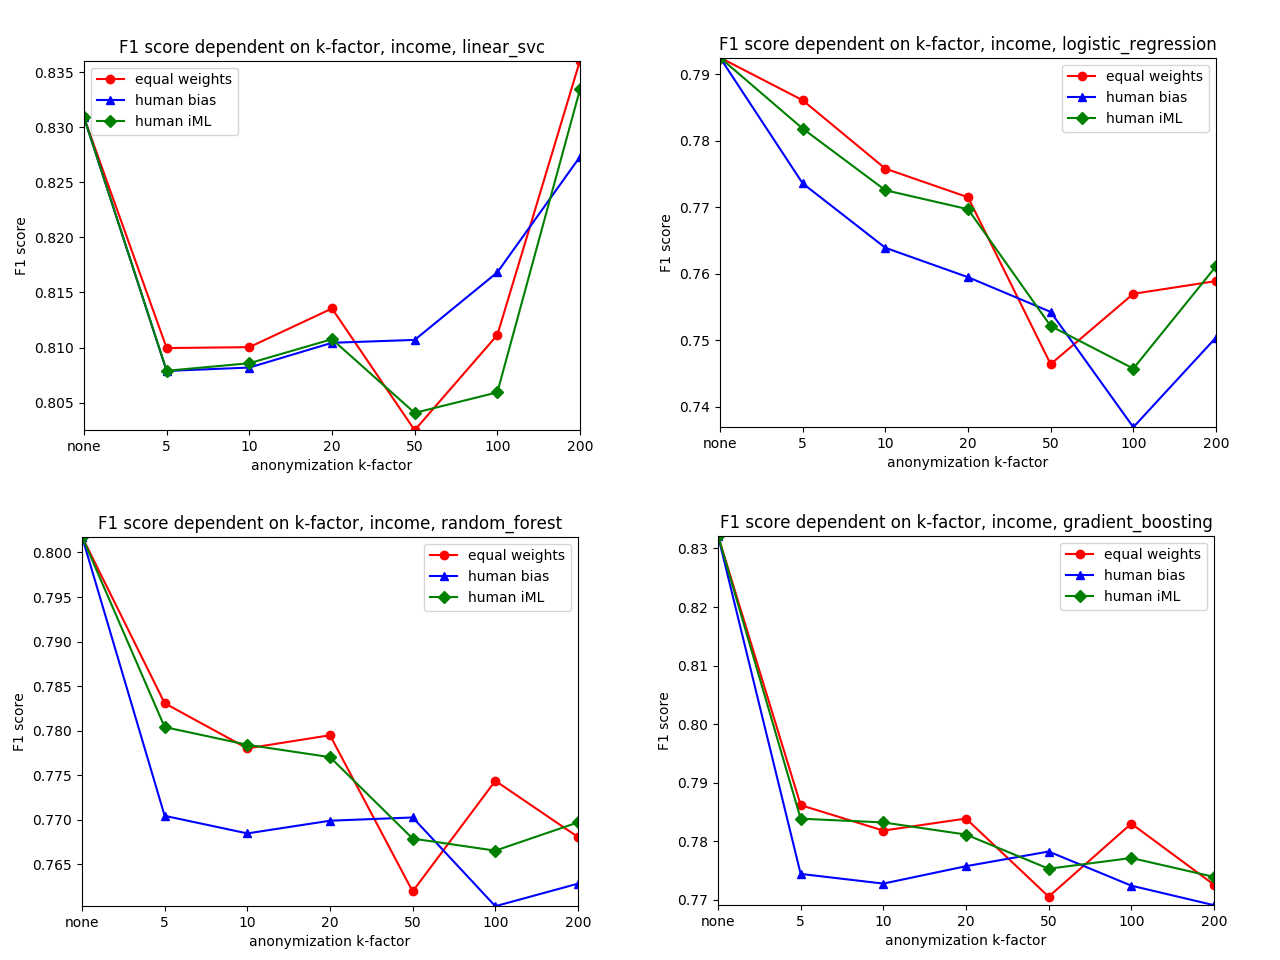
\includegraphics[width=1.0\textwidth]{figures/income.png}
		\caption{Results on...}
		\label{fig:results_income}
	\end{center}
\end{figure}

\begin{figure}[!h]
	\begin{center}
		\vspace{-1.0cm}
		\hspace*{-0.8cm}
		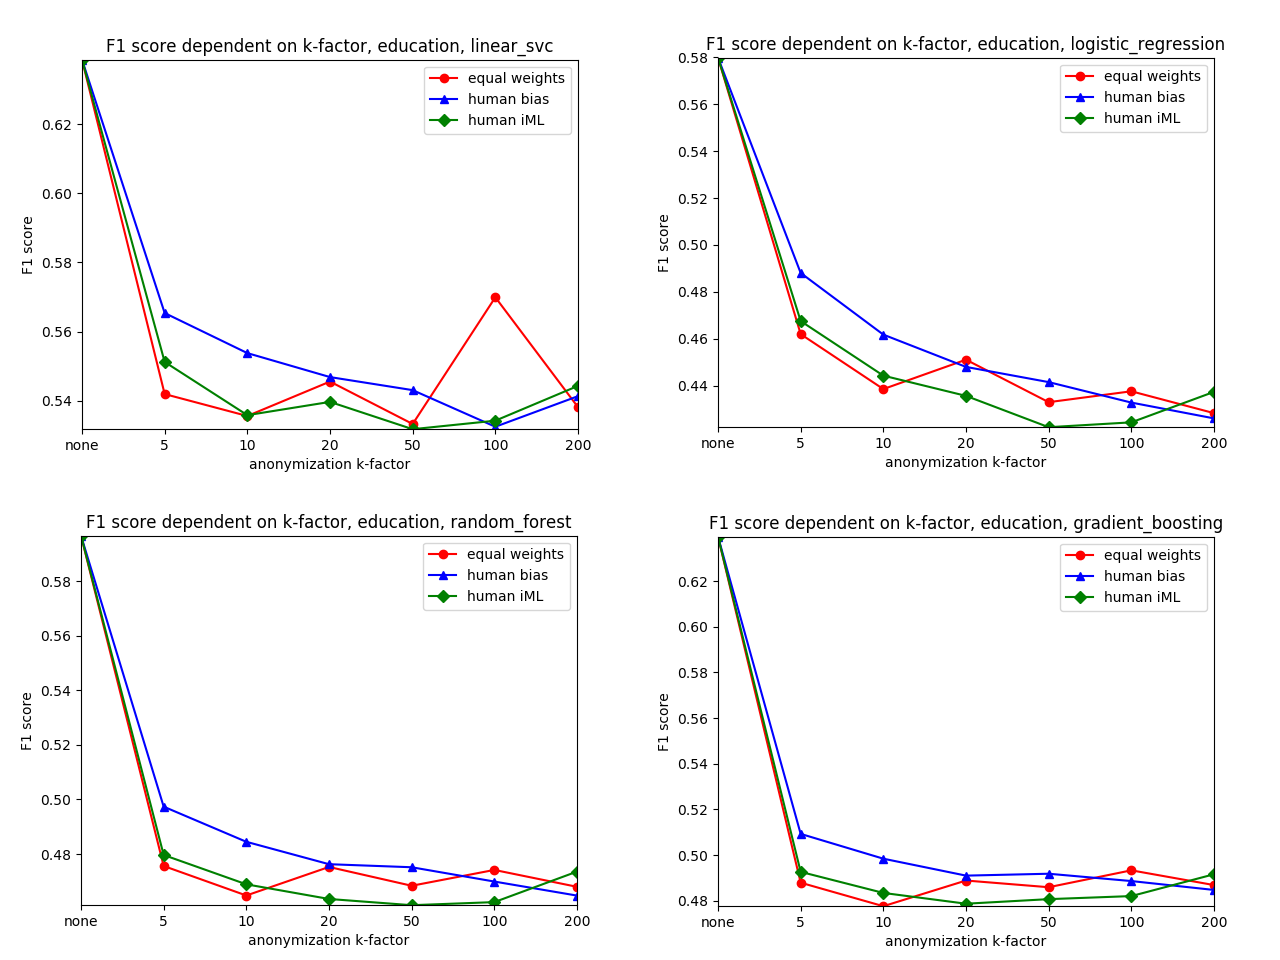
\includegraphics[width=1.0\textwidth]{figures/education_num.png}
		\caption{Results on...}
		\label{fig:results_education}
	\end{center}
\end{figure}

\begin{figure}[!h]
	\begin{center}
		\vspace{-1.0cm}
		\hspace*{-0.8cm}
		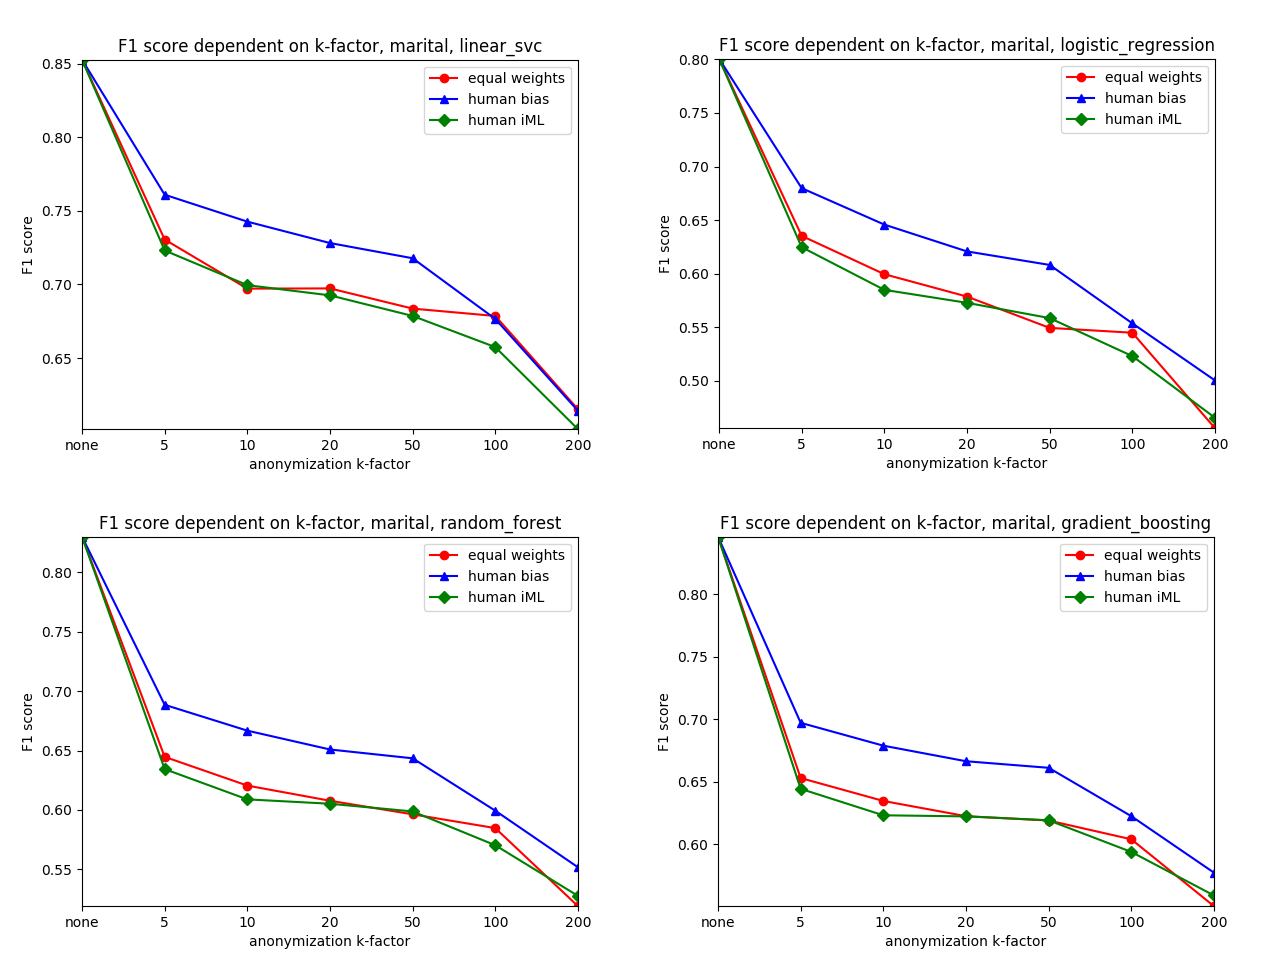
\includegraphics[width=1.0\textwidth]{figures/marital_status.png}
		\caption{Results on...}
		\label{fig:results_marital}
	\end{center}
\end{figure}



% ==================================
%		PROBLEMS & CHALLENGES
% ==================================
\section{Open problems \& future challenges}
\label{sect:op_fc}

\begin{itemize}
	\item \textbf{Explain the unexpected behavior} for...
\end{itemize}


% ==================================
%			CONCLUSION
% ==================================
\section{Conclusion}
\label{sect:conclusion}


\clearpage
\newpage

\bibliographystyle{plain}
\bibliography{references}

\end{document}

